
\chapter{Elementos Pós-Textuais}

\section{Índice Remissivo}

Pode ser construído de forma eficiente, simples e consistente com
o pacote \pacote{makeidx}. Vários textos descrevem como construir
um Índice Remissivo com este pacote, veja por exemplo,
\ttt{\LaTeX{} tintim por tintim}.

\section{Referências}

Todas as formas de construir referência com o \LaTeX{} são suportadas
pela classe \estilo, mas apenas três estão configuradas em opções de classe.
\begin{itemize}
	\item{\negri refkom}: é o padrão nas classes scrkook e estilo;
	\item{\negri refnum}: sistema de referência numérico, carrega o pacote
	\pacote{natbib};
	\item{\negri refaa}: sistema de referência autor-ano, carrega o pacote
	\pacote{natbib}.
\end{itemize}

Os comandos
\begin{tcolorbox}
\begin{lstlisting}
   \renewcommand{\bibname}{Referências}
   \bibliographystyle{unsrtnat}
   \bibliography{bibliografia}
\end{lstlisting}
\end{tcolorbox}
devem ser inseridos onde a lista de referências deve ser criada.
\begin{itemize}
\item O \cmc{renewcommand}{\coma{bibname}}$\{$Referências$\}$ define o
   título das referências. Sem esse comando o pacote babel traduzirá
   o título para Referências Bibliográficas, termo que ficou obsoleto
   por que atualmente existem referências que não são bibliográficas.
\item \cmc{bibliographystyle}{unsrtnat}: define o estilo de bibliografia, nesse 
caso o \textsf{unsrtnat} que pertence ao pacote natbib, mas você pode escolher 
outros que também atenda as normas.
\item \cmc{bibliography}{bibliografia}: carrega o arquivo
   bibliografia.bib, o banco de referências, o qual deve ficar
   na mesma pasta de seu arquivo .tex e deve ser feito segundo
   as regras do bibtex ou biber. Segue um exemplo mínimo de
   arquivo .bib segundo as regras do bib\TeX.
\end{itemize}

\begin{tcolorbox}[title={Exemplo de arquivo .bib}]
\begin{lstlisting}
@BOOK{casaliorio,
author = "Júnior, R. I.; Iório, V. M.;",
title = "Equações Diferenciais Parciais: Uma introdução",
edition = "2",
address = "Rio de Janeiro",
publisher = "IMPA",
year = "2010",
}
@book{Elon,
author       = {Elon Lages Lima},
title        = {Curso de An\'alise Volume 1},
address      = {Rio de Janeiro, Rio de Janeiro},
publisher    = {IMPA - Projeto Euclives},
edition      = {$11^a$},
isbn         = {85-244-0118-4},
year         = {2004},
}
@BOOK{briggs,
author = "Briggs, Willian L.;",
title = "A Multigrid Tutorial",
edition = "2",
address = "Philadelphia",
publisher = "SIAM",
year = "1987",
}
@ARTICLE{saad,
author = "SAAD, Y.,",
title = {Iterative Methods for Sparse Linear Systems},
journal = {PWS Publish-ing Company},
address = "Boston",
year = 1996,
}
\end{lstlisting}
\end{tcolorbox}

O arquivo .bib que gerou as referências deste manual é distribuído junto com a classe estilo, construa o seu a partir dele acrescentando os seus itens bibliográficos.

A citação é feita com o comando \cmc{cite}{apelido} ou \cmc{citet}{apelido} ou
outros que o pacote natbib oferece, mas apenas o \cmc{cite}{apelido} já é suficiente. O apelido é o primeiro nome do item no seu arquivo .bib. Para fazer referência ao primeiro item do exemplo de arquivo .bib dado deveria ser inserido o comando \cmc{cite}{casaliorio}, veja
\begin{tcolorbox}[title={Sistema de referenciação numérico: opção refnum}]
\begin{lstlisting}
   Segundo \cite{casaliorio}, as equações diferenciais parciais podem ser classificadas em hiperbólicas, parabólicas e elípticas.
\end{lstlisting}
\tcblower
Depois de compilado esse código produz

Segundo \cite{casaliorio}, as equações diferenciais parciais podem ser classificadas em hiperbólicas, parabólicas e elípticas.
\end{tcolorbox}

\begin{figure}[H]
   \resizebox{\textwidth}{!}{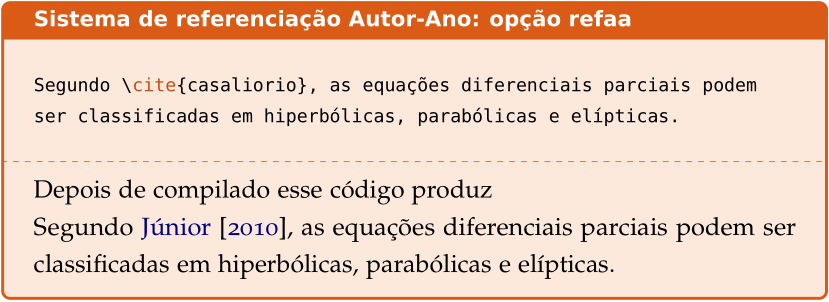
\includegraphics{Autor-Ano}}
\end{figure}

Observe que nos dois exemplos a citação é feita com o comando \cmc{cite}{casaliorio}, ou seja, é independente do estilo de bibliografia. Desta forma, para alterar a formatação de suas referências basta carregas um estilo diferente e compilar seu arquivo.

\subsubsection{Atenção}
Apenas as referências citadas no texto são incluídas na
lista de referências, ou seja, o \LaTeX\ previne esquecimentos
deliberados e impede que sejam incluídas nas referências
bibliografias que não foram citadas no texto.


\subsubsection{A lista de referências}

A lista de referências é criada na posição correspondente a inserção do comandos \com{bibliography} e sua primeira página recebe a mesma formatação da primeira página do sumário.

\section{Anexos e apêndices}
\begin{description}
\item[O que é um Anexo?]
	É um conjunto de informações complementares necessárias
    para a entendimento do trabalho ou parte dele.	
\item[O que é um Apêndice?]
	É um conjunto de informações suplementares acrescentado
    ao trabalho para suporte ou contextualização mas não
    necessário para o entendimento do trabalho ou parte dele.
\end{description}

\exemplo\,\, Seu trabalho usa fortemente resultados pouco conhecidos
ou extensos demais para serem inseridos no corpo do texto. No
final você pode inserir os tais resultados que constituirão um ou mais anexos.

\exemplo\,\, Seu trabalho aborda a vida de Charles Chaplin. No final você
pode inserir fotos de cartazes dos filmes dele, algumas de suas
frases famosas, fotografias dele. $\ldots$. Como essas informações
não são necessárias para o bom entendimento do seu trabalho elas
constituem um apêndice.

Note a diferença entre anexo e apêndice, o anexo contém informações
indispensáveis para a compreensão do trabalho enquanto o apêndice
contém informações acessórias e cuja ausência não comprometem a
compreensão do texto ou parte dele.

Na classe \estilo\ anexos são criados com o comando \com{anexo} e apêndices
são criados com o comando \com{apendice}, ambos utilizam o comando
\comando{appendix}, que é nativo da classe scrbook e não pode ser
carregado mais de uma vez no mesmo documento.

Para criar um anexo insira o comando \com{anexo}, depois dele todas
as ocorrêcias do comando \com{chapter} iniciarão um anexo.
\begin{tcolorbox}[title={Como criar anexos}]
	\begin{lstlisting}
	\anexo
	\chapter{Vida dura}
	\section{A vida gosta de quem gosta dela}
	\chapter{Você aprende}
	\section{Aprende que beijos não são contratos}
	\end{lstlisting}
	\tcblower
	
Depois de compilado esse código cria dois anexos: o Anexo I com
título Vida dura e a seção I.1 com título A vida gosta de quem gosta
dela, e o Anexo II com o título Você aprende e a seção II.1 com título
Aprende que beijos não são contratos
\end{tcolorbox}

Para criar um apêndice insira o comando \com{apendice},
depois dele todas as ocorrências do comando \com{chapter}
iniciarão um apêndice.
\begin{tcolorbox}[title={Como criar apêndice}]
	\begin{lstlisting}
	\apendice
	\chapter{Vida dura}
	\section{A vida gosta de quem gosta dela}
	\chapter{Você aprende}
	\section{Aprende que beijos não são contratos}
	\end{lstlisting}
	\tcblower
	
Depois de compilado esse código cria dois apêndices: o
Apêndice A com título Vida dura e a seção A.1 com título A
vida gosta de quem gosta dela, e o Apêndice B com o título
Você aprende e a seção B.1 com título Aprende que beijos
não são contratos
\end{tcolorbox}
\subsection{Apêndice sem anexo}
O apêndice deve vir depois do anexo. Para atender a essa norma
o comando \com{apendice} foi implementado de modo que só
funciona corretamente depois do comando \com{anexo}. Se
acontecer de o trabalho exigir apenas a inclusão de apêndices
deve-se carregar a opção de classe \ttt{apenas} e utilizar o
comando \com{apendice} normalmente para criar os apêndices.

